\section{Parametric Memory and Its Limits}

\begin{frame}{}
    \LARGE Research Frontiers: \textbf{Parametric Memory}

    \vspace{1em}
    \normalsize Where do facts live in a model, and can we update them or trace them?
\end{frame}

\begin{frame}{Where Do Facts Live?}
    \begin{columns}[T,onlytextwidth]
        \column{0.6\textwidth}
        \begin{itemize}\itemsep0.45em
            \item \textbf{2019:} a language model is already a knowledge base. BERT answers relational cloze queries with no fine-tuning.
            \item \textbf{2021:} feed-forward layers act as \emph{key-value memories}. Keys match input patterns. Values promote output tokens.
            \item \textbf{2022, causal tracing:} corrupt the subject, then restore one hidden state at a time. Facts localise to \textbf{MLPs in middle layers at the last subject token}. Later attention carries the fact to the output.
        \end{itemize}
        \column{0.38\textwidth}
        \centering
        \begin{adjustbox}{max width=\linewidth}\begin{tikzpicture}[font=\scriptsize, >=Stealth]
            \foreach \x in {0,...,4} { \foreach \y in {0,...,5} { \draw[gray!50] (0.8*\x,0.5*\y) rectangle (0.8*\x+0.72,0.5*\y+0.42); } }
            \draw[fill=darkorange!55] (1.6,1.0) rectangle (2.32,1.42);
            \draw[fill=darkorange!55] (1.6,1.5) rectangle (2.32,1.92);
            \draw[fill=darkorange!55] (1.6,2.0) rectangle (2.32,2.42);
            \draw[fill=KAUSTcyan!55] (3.2,2.0) rectangle (3.92,2.42);
            \draw[fill=KAUSTcyan!55] (3.2,2.5) rectangle (3.92,2.92);
            \draw[->, thick] (2.36,2.21) -- (3.16,2.21);
            \node[rotate=90] at (-0.35,1.45) {layers};
            \node[align=center] at (1.96,-0.4) {last subject\\token};
            \node[align=center] at (3.56,-0.4) {last\\token};
            \node[darkorange!80!black] at (1.2,3.3) {MLPs retrieve};
            \node[KAUSTcyan!70!black] at (3.4,3.3) {attention moves};
        \end{tikzpicture}\end{adjustbox}

        {\scriptsize Schematic of the causal-tracing finding.}
    \end{columns}
    \vspace{0.2em}
    \caveat{A useful picture, not an address map. Edits also succeed in layers other than the traced ones.}
    \src{Petroni et al., \href{https://arxiv.org/abs/1909.01066}{arXiv:1909.01066}. Geva, Schuster, Berant, Levy, \href{https://arxiv.org/abs/2012.14913}{arXiv:2012.14913}. Meng, Bau, Andonian, Belinkov, ``ROME,'' \href{https://arxiv.org/abs/2202.05262}{arXiv:2202.05262}. Hase, Bansal, Kim, Ghandeharioun, \href{https://arxiv.org/abs/2301.04213}{arXiv:2301.04213}.}
\end{frame}

\begin{frame}{How Much Fits? Two Bits per Parameter}
    \begin{columns}[T,onlytextwidth]
        \column{0.5\textwidth}
        \centering
        \small
        \renewcommand{\arraystretch}{1.15}
        \footnotesize\setlength{\tabcolsep}{3pt}\begin{adjustbox}{max width=\linewidth}\begin{tabular}{lc}
            \toprule
            \textbf{Condition (synthetic data)} & \textbf{Capacity} \\
            \midrule
            \rowcolor{KAUSTcyan!12} Each fact seen 1,000 times & 2 bits per weight \\
            Each fact seen 100 times & about 1 bit \\
            Quantised to int8 & unchanged \\
            Quantised to int4 & about 0.7 bit \\
            MoE, 32 experts & 1.3x lower \\
            7/8 of the data is junk & 20x lower \\
            Junk, with a domain tag on good data & 2x lower \\
            \bottomrule
        \end{tabular}\end{adjustbox}
        \column{0.48\textwidth}
        \begin{itemize}\itemsep0.45em
            \item A 7B model can hold about 14B bits. \textbf{Capacity is bounded, and exposure matters.}
            \item \textbf{What fails even when it fits:}
            \begin{itemize}\itemsep0.2em
                \item \emph{The long tail.} Accuracy tracks how many pre-training documents mention the fact. Scaling does not fix rare facts. Retrieval does.
                \item \emph{The reversal curse.} Trained on ``A is B'', GPT-4 names a celebrity's parent 79\% of the time, and the reverse 33\%.
            \end{itemize}
        \end{itemize}
    \end{columns}
    \vspace{0.2em}
    \src{Allen-Zhu, Li, ``Physics of Language Models: Part 3.3, Knowledge Capacity Scaling Laws,'' \href{https://arxiv.org/abs/2404.05405}{arXiv:2404.05405}. Kandpal et al., \href{https://arxiv.org/abs/2211.08411}{arXiv:2211.08411}. Mallen et al., \href{https://arxiv.org/abs/2212.10511}{arXiv:2212.10511}. Berglund et al., ``The Reversal Curse,'' \href{https://arxiv.org/abs/2309.12288}{arXiv:2309.12288}.}
\end{frame}

\begin{frame}{Editing the Weights: ROME, MEMIT, AlphaEdit}
    \begin{itemize}\itemsep0.3em
        \item If a fact is a key-value pair in an MLP, write a new one. \textbf{ROME} applies a rank-one update. \textbf{MEMIT} solves a least-squares problem for thousands of facts.
        \item Both trade new knowledge $(K_1,V_1)$ against preserved knowledge $(K_0,V_0)$. \textbf{AlphaEdit} removes the trade: project the update onto the \emph{null space} of the preserved keys, so that $(W+\Delta P)\,K_0 = WK_0$.
    \end{itemize}
    \centering
    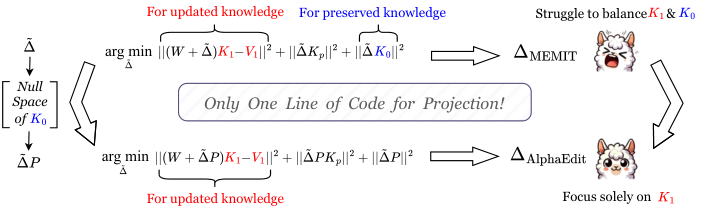
\includegraphics[width=0.78\linewidth,height=0.24\textheight,keepaspectratio]{images/research-frontiers/alphaedit_fig_method.png}
    \begin{center}
    \small
    \begin{adjustbox}{max width=\linewidth}\begin{tabular}{lcccc}
        \toprule
        \textbf{LLaMA3-8B, sequential edits} & \textbf{Efficacy} & \textbf{Generalisation} & \textbf{Specificity} & \textbf{Fluency} \\
        \midrule
        MEMIT & 65.65 & 64.65 & 51.56 & 437.43 \\
        \rowcolor{KAUSTcyan!12} AlphaEdit & 98.90 & 94.22 & 67.88 & 622.49 \\
        \bottomrule
    \end{tabular}\end{adjustbox}
    \end{center}
    \src{Meng et al., ``ROME,'' \href{https://arxiv.org/abs/2202.05262}{arXiv:2202.05262}. Meng et al., ``MEMIT,'' \href{https://arxiv.org/abs/2210.07229}{arXiv:2210.07229}. Fang et al., ``AlphaEdit,'' ICLR 2025, \href{https://arxiv.org/abs/2410.02355}{arXiv:2410.02355}, method figure and Table 1.}
\end{frame}

\begin{frame}{Why Editing Is Not a Freshness Solution}
    \begin{columns}[T,onlytextwidth]
        \column{0.62\textwidth}
        \begin{itemize}\itemsep0.4em
            \item \textbf{Consequences do not propagate.} ROME recalls the edited fact 88.3\% of the time, and answers multi-hop questions that depend on it \alert{7.4\%} of the time. Unedited: 40.5\%.
            \item \textbf{In-context beats in-weights.} Giving the new fact in the prompt scores 82.8 on ripple effects. ROME scores 60.8.
            \item \textbf{Edits pile up, then the model collapses.} MEMIT falls off a cliff after about 1,400 edits (right).
            \item \textbf{At real volume it fails.} Wikipedia produced 502,382 updates in five months. Editors collapse within a few hundred.
        \end{itemize}
        \column{0.36\textwidth}
        \centering
        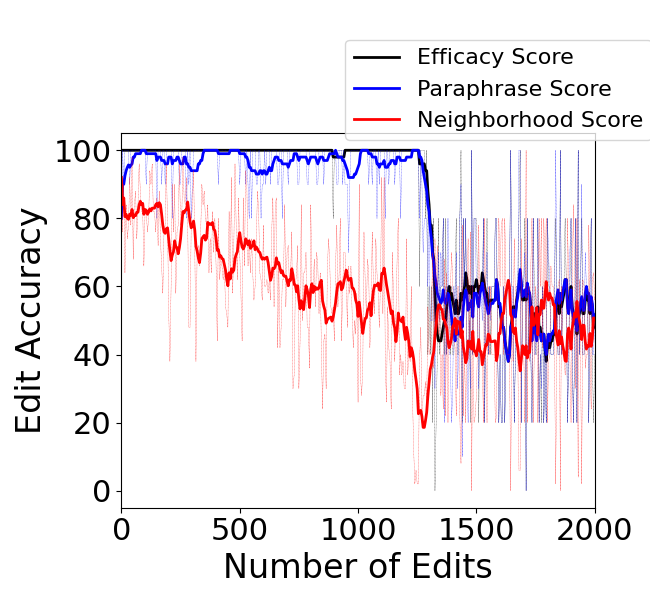
\includegraphics[width=\linewidth,height=0.45\textheight,keepaspectratio]{images/research-frontiers/gupta_memit_editing_score.png}

        {\scriptsize MEMIT on GPT-J.}
    \end{columns}
    \vspace{0.2em}
    \takeaway{Editing is a surgical, low-volume tool and an interpretability probe. It is not how a model stays current.}
    \src{Zhong, Wu, Manning, Potts, Chen, ``MQuAKE,'' \href{https://arxiv.org/abs/2305.14795}{arXiv:2305.14795}. Cohen et al., \href{https://arxiv.org/abs/2307.12976}{arXiv:2307.12976}. Figure: Gupta, Rao, Anumanchipalli, \href{https://arxiv.org/abs/2401.07453}{arXiv:2401.07453}. Thede et al., ``WikiBigEdit,'' \href{https://arxiv.org/abs/2503.05683}{arXiv:2503.05683}.}
\end{frame}

\begin{frame}{Memory Layers: a Second Axis of Sparsity}
    \begin{itemize}\itemsep0.3em
        \item Day 1's MoE made \emph{computation} sparse. Memory layers make \emph{storage} sparse: a huge trainable key-value table, of which each token reads only a few rows:
        $I=\mathrm{TopK}(Kq)$, \ $y=\mathrm{Softmax}(K_I\,q)\,V_I$.
    \end{itemize}
    \begin{center}
    \footnotesize
    \renewcommand{\arraystretch}{1.15}
    \begin{adjustbox}{max width=\linewidth}\begin{tabular}{>{\raggedright\arraybackslash}p{3.6cm}>{\raggedright\arraybackslash}p{9.6cm}}
        \toprule
        \textbf{System} & \textbf{What it shows} \\
        \midrule
        Memory Layers at Scale (Meta, Dec 2024) & up to 128B memory parameters. Better than Llama-2-7B on factual QA (27.06 against 25.10), and \emph{worse} on MMLU (63.04 against 66.00) \\
        \rowcolor{KAUSTcyan!12} Engram (2026) & hashed N-gram embeddings, looked up in $O(1)$. Best with 20 to 25\% of the sparse budget in memory. A 100B table in host RAM costs 2.8\% throughput \\
        \bottomrule
    \end{tabular}\end{adjustbox}
    \end{center}
    \begin{itemize}\itemsep0.3em
        \item \textbf{Why it matters for updates.} Tune only the memory slots that new facts activate. At equal new knowledge, old QA accuracy drops 89\% with full fine-tuning, 71\% with LoRA, and \textbf{11\%} this way.
    \end{itemize}
    \caveat{No verified evidence that a 2026 frontier model ships these layers.}
    \src{Berges et al., ``Memory Layers at Scale,'' \href{https://arxiv.org/abs/2412.09764}{arXiv:2412.09764}. Cheng et al., ``Conditional Memory via Scalable Lookup,'' \href{https://arxiv.org/abs/2601.07372}{arXiv:2601.07372}. Lin et al., ``Continual Learning via Sparse Memory Finetuning,'' \href{https://arxiv.org/abs/2510.15103}{arXiv:2510.15103}.}
\end{frame}

\begin{frame}{Weights, Explicit Memory or Plain Text? A Cost Model}
    \begin{columns}[T,onlytextwidth]
        \column{0.48\textwidth}
        \centering
        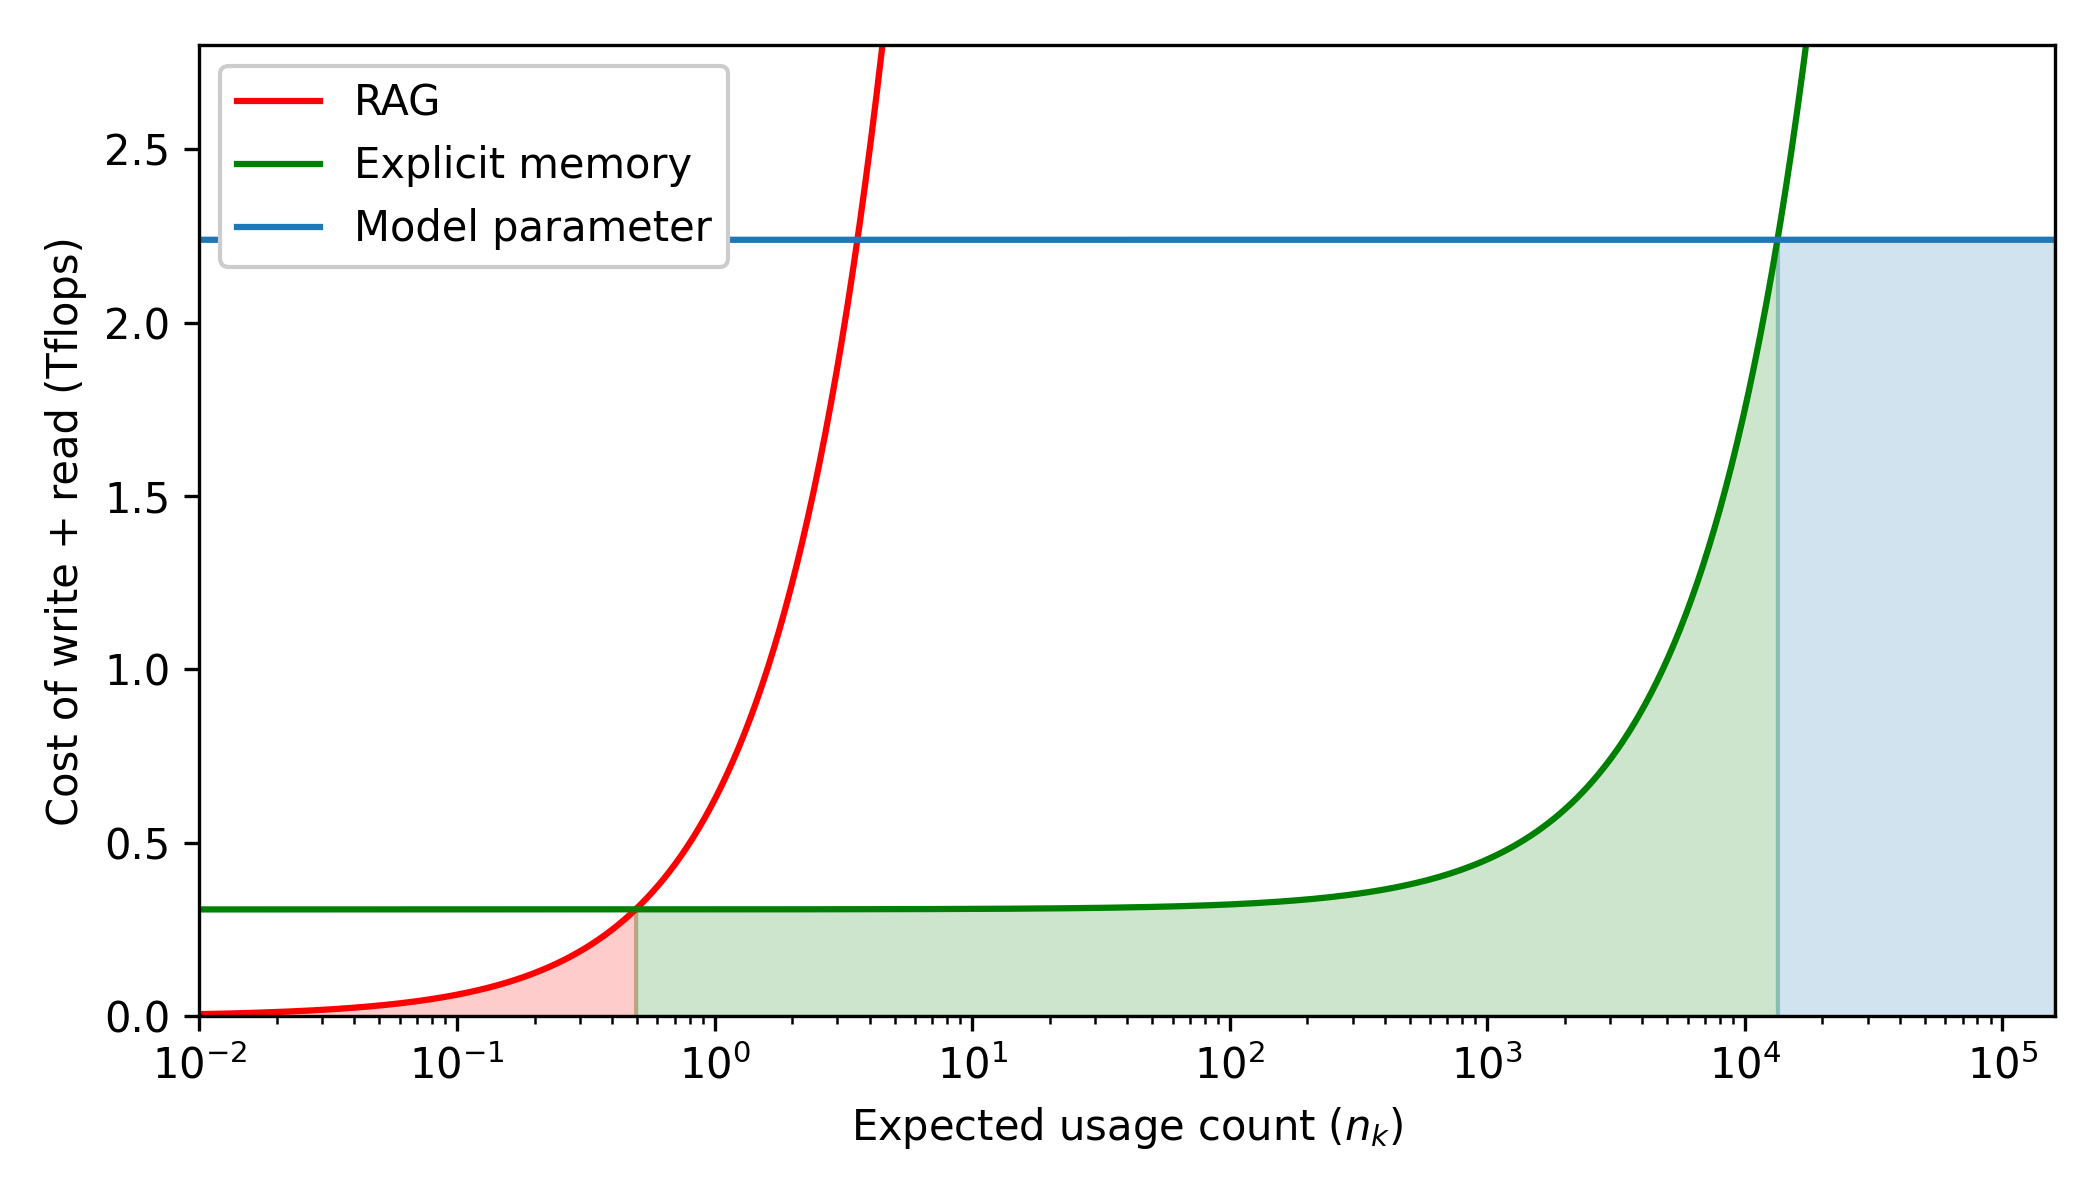
\includegraphics[width=\linewidth,height=0.5\textheight,keepaspectratio]{images/research-frontiers/memory3_fig4_total_cost.png}
        \column{0.5\textwidth}
        \begin{itemize}\itemsep0.4em
            \item Knowledge $k$ is written once and read $n_k$ times. Choose the format $m$ that minimises
            \[
                \text{cost}_{\text{write}}(k,m) + n_k\,\text{cost}_{\text{read}}(k,m)
            \]
            \item \textbf{Plain text} (RAG): free to write, costly on every read.
            \item \textbf{Parameters:} costly to write, free to read.
            \item \textbf{Explicit memory} (stored sparse KV of reference text) wins in between: from about 0.5 to 13,400 uses.
        \end{itemize}
    \end{columns}
    \vspace{0.2em}
    \takeaway{Memory is a spectrum. Retrieval-free and retrieval-based are its two ends, not rivals.}
    \src{Yang et al., ``Memory3: Language Modeling with Explicit Memory,'' \href{https://arxiv.org/abs/2407.01178}{arXiv:2407.01178}, Figure 4. Zhoubian, Zhang, Kharlamov, Tang, ``Memory for Large Language Models,'' \href{https://arxiv.org/abs/2607.25380}{arXiv:2607.25380}.}
\end{frame}

\begin{frame}{Memory-Augmented Networks: Learning to Memorise at Test Time}
    \centering
    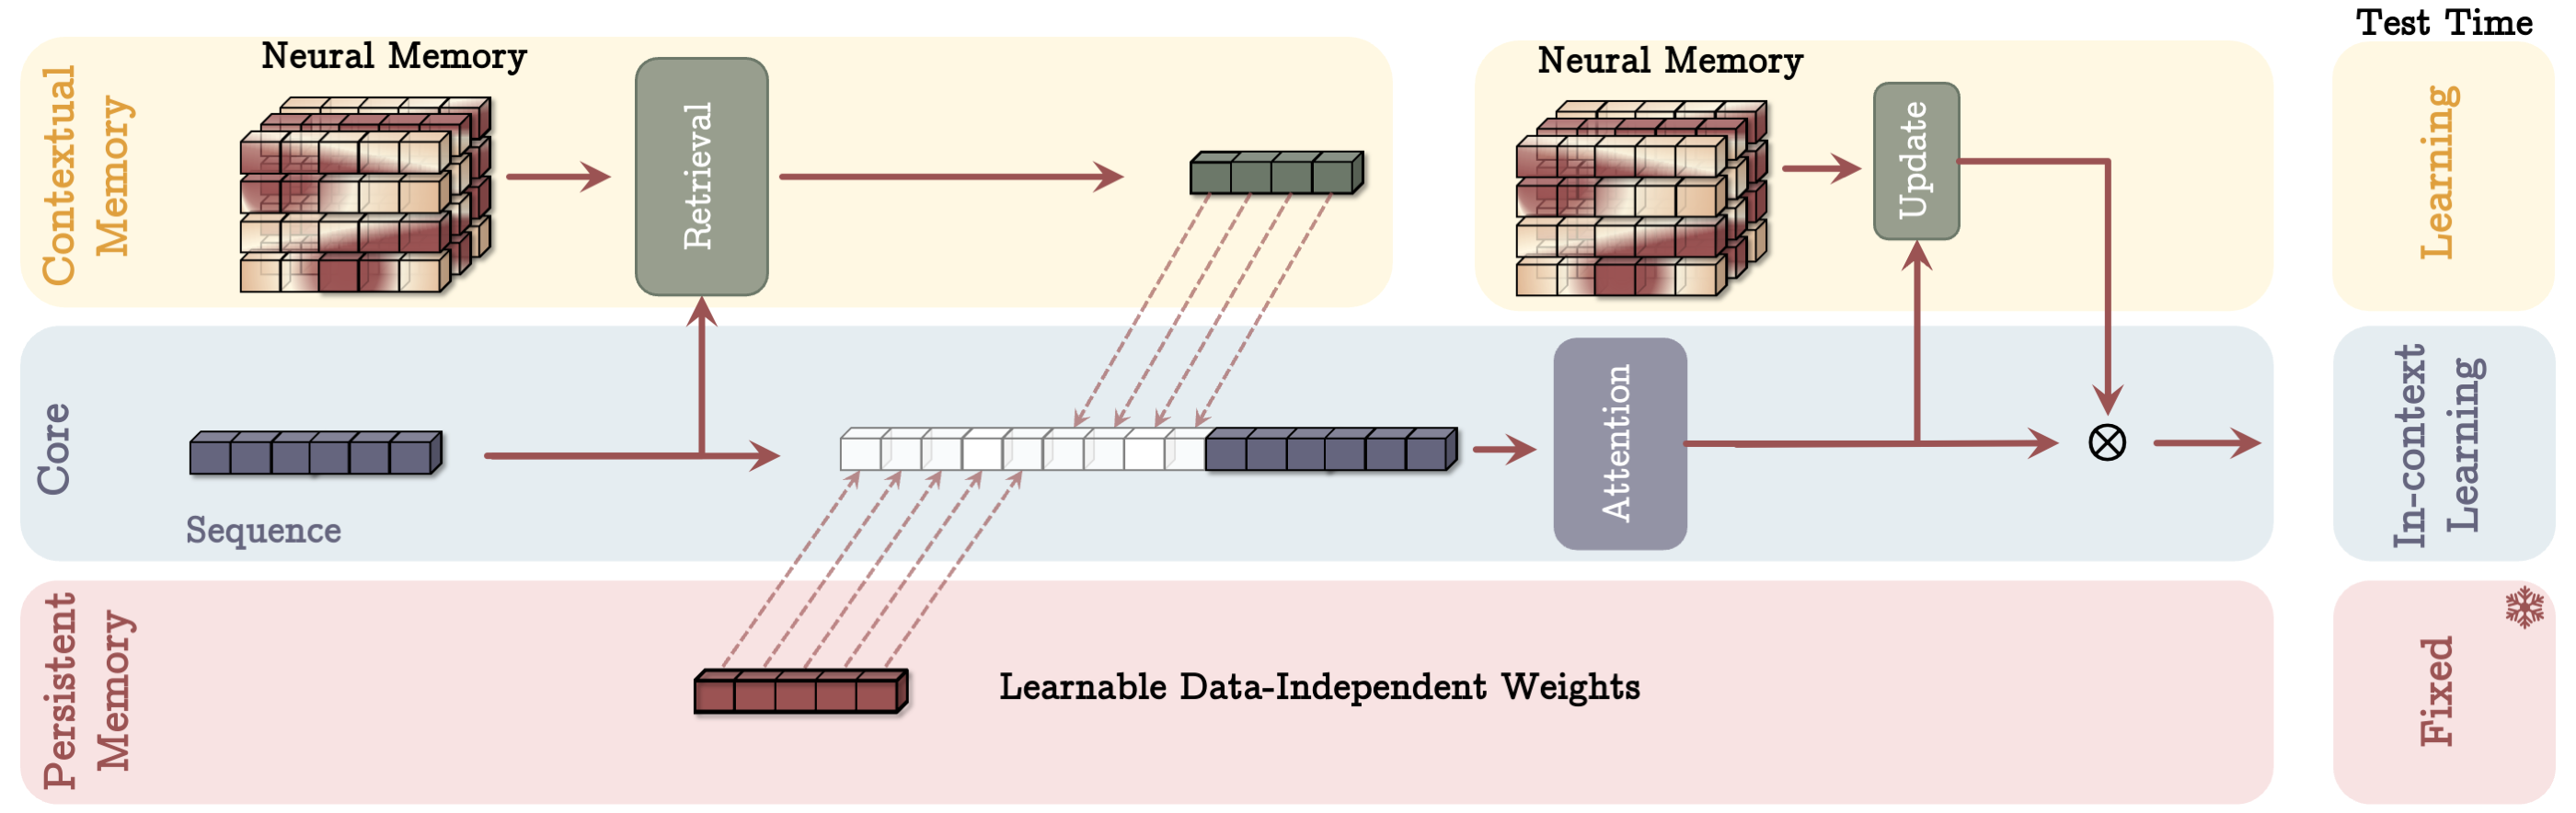
\includegraphics[width=0.9\linewidth,height=0.3\textheight,keepaspectratio]{images/research-frontiers/titans_fig2_mac_architecture.png}
    \begin{itemize}\itemsep0.3em
        \item \textbf{Titans:} a small network $\mathcal{M}$ is the long-term memory. It is \emph{trained during inference} to map keys to values:
        \[
            \mathcal M_t=(1-\alpha_t)\,\mathcal M_{t-1}+S_t, \qquad S_t=\eta_t S_{t-1}-\theta_t\nabla\lVert\mathcal M_{t-1}(k_t)-v_t\rVert_2^2
        \]
        \item This is Day 1's delta rule with \textbf{momentum} $\eta_t$, \textbf{forgetting} $\alpha_t$ and a \textbf{deep} memory in place of a matrix.
        \item Needle retrieval at 16K tokens: Mamba2 5.4, DeltaNet 71.4, Titans 98.4.

    \end{itemize}
    \src{Behrouz, Zhong, Mirrokni, ``Titans: Learning to Memorize at Test Time,'' \href{https://arxiv.org/abs/2501.00663}{arXiv:2501.00663}, architecture figure, Eqs. 9 to 14 and Table 2. Note: all results are below about 1B parameters, and no production model is known to ship it.}
\end{frame}

\begin{frame}{Limit 1: Freshness}
    \begin{center}
    \small
    \renewcommand{\arraystretch}{1.2}
    \begin{adjustbox}{max width=\linewidth}\begin{tabular}{>{\raggedright\arraybackslash}p{4.4cm}>{\raggedright\arraybackslash}p{8.9cm}}
        \toprule
        \textbf{Failure} & \textbf{Evidence} \\
        \midrule
        The model does not know where its knowledge ends & RedPajama reports a cutoff of January 2023. Its \emph{effective} cutoff, measured on dated Wikipedia, is mid-2019 \\
        Fine-tuning is a poor way to add facts & RAG consistently beats unsupervised fine-tuning \\
        Learning new facts raises hallucination & unknown facts are learned slowly, and hallucination rises linearly as they are learned \\
        Putting the index in the weights does not help & generative retrieval beats a dual encoder on small corpora, and stalls at millions of passages \\
        \bottomrule
    \end{tabular}\end{adjustbox}
    \end{center}
    \begin{itemize}\itemsep0.35em
        \item Old pages inside new crawls pull the effective cutoff backwards.
        \item \textbf{``Retrieval-free'' inherits every limit of parametric memory}: staleness, bounded capacity, no provenance.
    \end{itemize}
    \src{Cheng et al., ``Dated Data,'' \href{https://arxiv.org/abs/2403.12958}{arXiv:2403.12958}. Ovadia et al., \href{https://arxiv.org/abs/2312.05934}{arXiv:2312.05934}. Gekhman et al., \href{https://arxiv.org/abs/2405.05904}{arXiv:2405.05904}. Tay et al., ``DSI,'' \href{https://arxiv.org/abs/2202.06991}{arXiv:2202.06991}. Pradeep et al., EMNLP 2023.}
\end{frame}

\begin{frame}{Limit 2: Attribution}
    \begin{itemize}\itemsep0.5em
        \item \textbf{Question:} which source supports this sentence? A parametric answer carries none.
        \item \textbf{Ask the model to cite.} Even the best models lack complete citation support \alert{50\%} of the time on long-form questions.
        \item \textbf{Ask the training data, causally.} Influence functions scale to a 52B model. Influence falls to near zero when the order of key phrases is flipped, which echoes the reversal curse.
        \item \textbf{Ask the training data, verbatim.} OLMoTrace matches output spans against all 4.6T training tokens in real time. It needs fully open data, and it shows overlap, \emph{not} a cause.
    \end{itemize}
    \vspace{0.3em}
    \takeaway{No method gives a faithful, cheap, per-claim source for a parametric answer from a closed-data model. This is the structural argument for retrieval and explicit memory.}
    \src{Gao, Yen, Yu, Chen, ``ALCE,'' \href{https://arxiv.org/abs/2305.14627}{arXiv:2305.14627}. Grosse, Bae et al., \href{https://arxiv.org/abs/2308.03296}{arXiv:2308.03296}. Liu et al., ``OLMoTrace,'' \href{https://arxiv.org/abs/2504.07096}{arXiv:2504.07096}, and Ai2 blog (2025).}
\end{frame}

\begin{frame}{Parametric Memory: What to Remember}
    \begin{itemize}\itemsep0.55em
        \item Facts sit mostly in feed-forward layers, at about \textbf{2 bits per parameter}, and only if seen often enough.
        \item \textbf{Editing} recalls the edited fact, fails on its consequences, and collapses after many edits.
        \item \textbf{Memory layers} and \textbf{test-time memory} move knowledge into addressable, updatable stores. Not yet in production.
        \item \textbf{Freshness:} models do not know their own cutoff, and learning new facts raises hallucination.
        \item \textbf{Attribution:} citations are incomplete half the time, and tracing is verbatim, not causal.
    \end{itemize}
    \vspace{0.4em}
    \takeaway{\textbf{Next.} A bounded, stale memory with no provenance will sometimes be asked what it does not know. Why does it answer anyway?}
\end{frame}
